%


\documentclass[twoside]{article}
\setlength{\oddsidemargin}{0.25 in}
\setlength{\evensidemargin}{-0.25 in}
\setlength{\topmargin}{-0.6 in}
\setlength{\textwidth}{6.5 in}
\setlength{\textheight}{8.5 in}
\setlength{\headsep}{0.75 in}
\setlength{\parindent}{0 in}
\setlength{\parskip}{0.1 in}

%
% ADD PACKAGES here:
%

\usepackage{amsmath,amsfonts,graphicx}

%
\newcounter{lecnum}
\renewcommand{\thepage}{\thelecnum-\arabic{page}}
\renewcommand{\thesection}{\thelecnum.\arabic{section}}
\renewcommand{\theequation}{\thelecnum.\arabic{equation}}
\renewcommand{\thefigure}{\thelecnum.\arabic{figure}}
\renewcommand{\thetable}{\thelecnum.\arabic{table}}

%
% The following macro is used to generate the header.
%
\newcommand{\lecture}[4]{
   \pagestyle{myheadings}
   \thispagestyle{plain}
   \newpage
   \setcounter{lecnum}{#1}
   \setcounter{page}{1}
   \noindent
   \begin{center}
   \framebox{
      \vbox{\vspace{2mm}
    \hbox to 6.28in { {\bf EE302 - Feedback Systems
	\hfill Spring 2019} }
       \vspace{4mm}
       \hbox to 6.28in { {\Large \hfill Lecture #1 \hfill} }
       \vspace{2mm}
       \hbox to 6.28in { {\it Lecturer: #2 \hfill } }
      \vspace{2mm}}
   }
   \end{center}
   \markboth{Lecture #1}{Lecture #1}

   \vspace*{4mm}
}
%
\renewcommand{\cite}[1]{[#1]}
\def\beginrefs{\begin{list}%
        {[\arabic{equation}]}{\usecounter{equation}
         \setlength{\leftmargin}{2.0truecm}\setlength{\labelsep}{0.4truecm}%
         \setlength{\labelwidth}{1.6truecm}}}
\def\endrefs{\end{list}}
\def\bibentry#1{\item[\hbox{[#1]}]}

%Use this command for a figure; it puts a figure in wherever you want it.
%usage: \fig{NUMBER}{SPACE-IN-INCHES}{CAPTION}
\newcommand{\fig}[3]{
			\vspace{#2}
			\begin{center}
			Figure \thelecnum.#1:~#3
			\end{center}
	}
% Use these for theorems, lemmas, proofs, etc.
\newtheorem{theorem}{Theorem}[lecnum]
\newtheorem{lemma}[theorem]{Lemma}
\newtheorem{proposition}[theorem]{Proposition}
\newtheorem{claim}[theorem]{Claim}
\newtheorem{corollary}[theorem]{Corollary}
\newtheorem{definition}[theorem]{Definition}
\newenvironment{proof}{{\bf Proof:}}{\hfill\rule{2mm}{2mm}}

% **** IF YOU WANT TO DEFINE ADDITIONAL MACROS FOR YOURSELF, PUT THEM HERE:

\begin{document}

% Lecture Details
\lecture{18}{Asst. Prof. M. Mert Ankarali}

\par

\section{The Bode Plot}

Previously, we showed how to illustrate the frequency response
function of an LTI system, $G(j \omega)$, using the polar plot
and the Nyquist plot. In the Bode Plot gain, $| G(j \omega) |$ and phase
response, $\angle [ G(j \omega) ]$, of the system are illustrated
separately as a function of frequency, $\omega$. In both diagrams
logarithmic scale is used for frequency axis. On the other hand,
in magnitude axis we use a special logarithmic scale in dB units,
where as for phase axis we use linear scale. Specifically Magnitude 
in dB scale, $M_{dB}$ and phase response, $\phi$ of a transfer
function, $G( j \omega)$ are computed as

\begin{align*}
 M_{dB}(\omega) &= 20 \mathrm{log}_{10} | G( j \omega ) |
  \\
  \phi(\omega) &= \angle [ G( j \omega )  ]
\end{align*}

Now let's write $G(s)$ in pole-zero-gain form and analyze the
magnitude (dB) and phase functions

\begin{align*}
  G(s) =& K \frac{ (s - z_1) \cdots (s - z_N) }{ (s - p_1) \cdots (s -
  p_N) }
\\
,
 \\
  M_{dB}\lbrace G(s) \rbrace =& 20 \mathrm{log}_{10} | G( j \omega ) | 
  \\
  =& 20 \mathrm{log}_{10} K + \left[ 20 \mathrm{log}_{10} | (j \omega
    - z_1) |  + \cdots + 20 \mathrm{log}_{10} (j \omega - z_N) \right]
    \\
    & - \left[ 20 \mathrm{log}_{10} | (j \omega
    - p_1) |  + \cdots + 20 \mathrm{log}_{10} (j \omega - p_M) \right]
      \\
  =& K_{dB} + \left[ M_{dB} \lbrace s - z_1 \rbrace \cdots M_{dB}
     \lbrace s - z_N \rbrace \right]
     - \left[ M_{dB} \lbrace s - p_1 \rbrace \cdots M_{dB}
     \lbrace s - p_M \rbrace \right]
\\
,
\\
  \phi \lbrace G(s) \rbrace &= \angle [ G( j \omega )  ]
\\
     &=  \left( \angle [ j \omega - z_1) ]  + \cdots + \angle [ j
       \omega - z_N ] \right) - \left( \angle [ j \omega - p_1 ]  +
       \cdots + \angle [ j \omega - p_M] \right)
\\&=  \left( \phi \lbrace s - z_1 \rbrace + \cdots + \phi \lbrace s -
    z_N \rbrace \right) - \left( \phi \lbrace s - p_1 \rbrace  +
       \cdots + \phi \lbrace s- p_M \rbrace \right)
\end{align*}

In conclusion, in order to obtain a bode diagram, we can 
first find phase and magnitude (dB) arguments associated 
with each pole/zero/gain separately for a given frequency.
After that, final magnitude (dB) and phase arguments of $G(s)$
are found by simply adding (and subtracting) the individual components.

\newpage

\textbf{Bode Plots of $s$ and $\frac{1}{s}$:} Let's write the
magnitude and phase functions 

\begin{align*}
s \ \Rightarrow \  M_{dB}(\omega) &= 20 \mathrm{log}_{10} ( \omega ) \quad \& \quad \phi (\omega) = 90^0 
                                                        \\
\frac{1}{s} \ \Rightarrow \ M_{dB} ( \omega ) &= - 20 \mathrm{log}_{10} ( \omega ) \quad \& \quad \phi (\omega) = -90^0 
\end{align*}

If we illustrate the responses in bode plot, we obtain the following Figure

\vspace{6 pt}

  \begin{minipage}[h]{1\linewidth}
    \begin{center}
      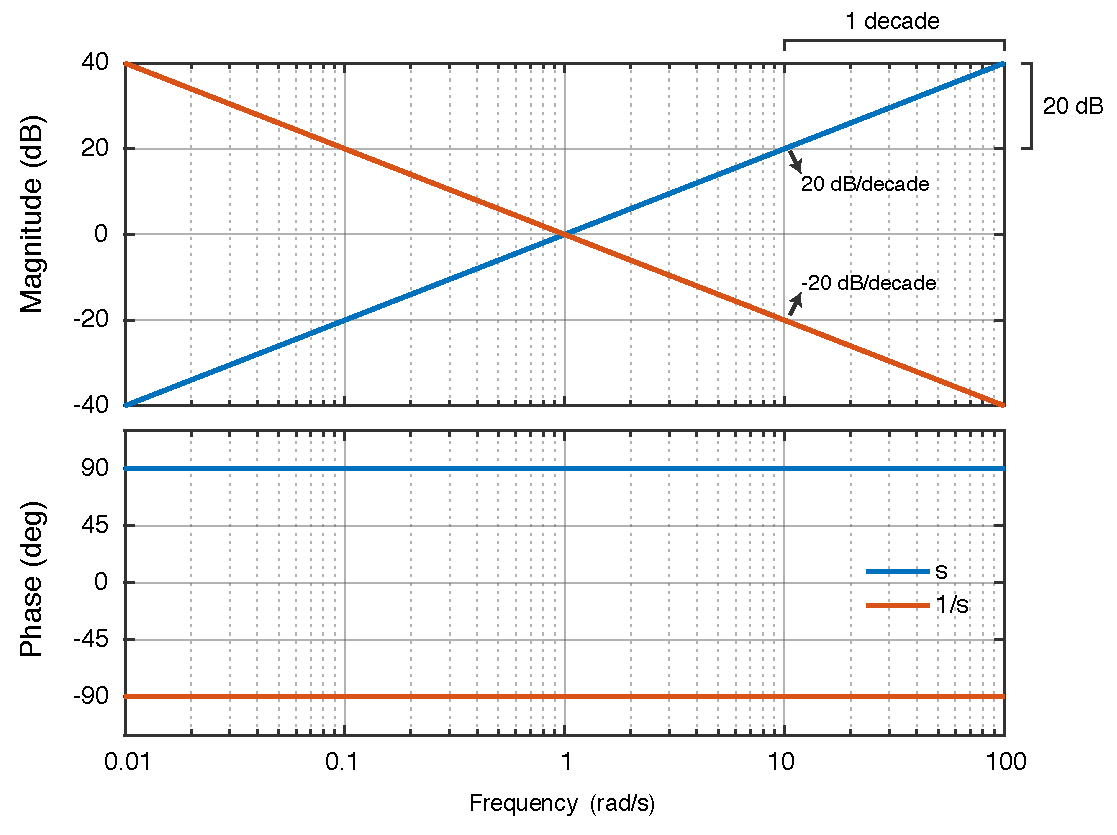
\includegraphics[width=0.8\textwidth]{bode_DandI}
    \end{center}
  \end{minipage}

\vspace{6pt}

\subsection*{Bode Plots of First-Order Forms}

First let's analyze the phase and magnitude (dB) response of $G(s) = s + 1$
%
\begin{align*}
  M_{dB} (\omega) &= 20 \, \mathrm{log}_{10} | G( j \omega) | = 20 \, \mathrm{log}_{10} \left( \omega^2 + 1 \right)^{1/2} = 10 \, \mathrm{log}_{10} \left( \omega^2 + 1 \right)
  \\
  \phi(\omega) &= \arctan \omega                                    
\end{align*}
%
Now we will approximate the gain and phase curves using piece-wise continuous straight lines. 
Firs approximate the magnitude response
%
\begin{align*}
  \mathrm{Low-Frequency} \ \Rightarrow \ M_{dB}(\omega)  &\approx 0 \
                                                   \mathrm{dB} \\
  \mathrm{High-Frequency} \ \Rightarrow \ M_{dB}(\omega)  &\approx 20 \,
                                                    \mathrm{log}_{10} ( \omega )
\end{align*}
%
Note that high-frequency and low-frequency approximations intersect at
$\omega = 1 \ rad/s$ and $M_{dB} = 0 \ \mathrm{dB}$ point. Now 
let's approximate the phase response
%
\begin{align*}
  \mathrm{Low-Frequency} \ \Rightarrow \ \phi  &\approx 0^o  \\
  \mathrm{High-Frequency} \ \Rightarrow \ \phi &\approx 90^o \\
  \mathrm{Medium-Frequency} \ \Rightarrow \ \phi & \approx 45^0 + 45^0 \mathrm{log}_{10} ( \omega)
\end{align*}
%
Note that, low-frequency and mid-frequency approximations intersect when $\omega = 0.1 \ rad/s$,
whereas high-frequency and mid-frequency approximations intersect when $\omega = 10 \ rad/s$.
The corner frequency of this ``system'' is $\omega_c = 1 \ rad/s$. Note that it is very easy to obtain 
the bode approximations of $G(s) = \frac{1}{s+1}$, if we know the bode approximations of $G(s) = s+1$. We
simple multiply both magnitude (dB) and phase responses of $s+1$ with $(-1)$. The figure below
illustrates the original bode plots (solid curves) of $G_1(s) = (s+1)$ and $G_2(s) = \frac{1}{s+1}$ as well as
their approximations (dashed lines). 

\vspace{6 pt}

  \begin{minipage}[h]{1\linewidth}
    \begin{center}
      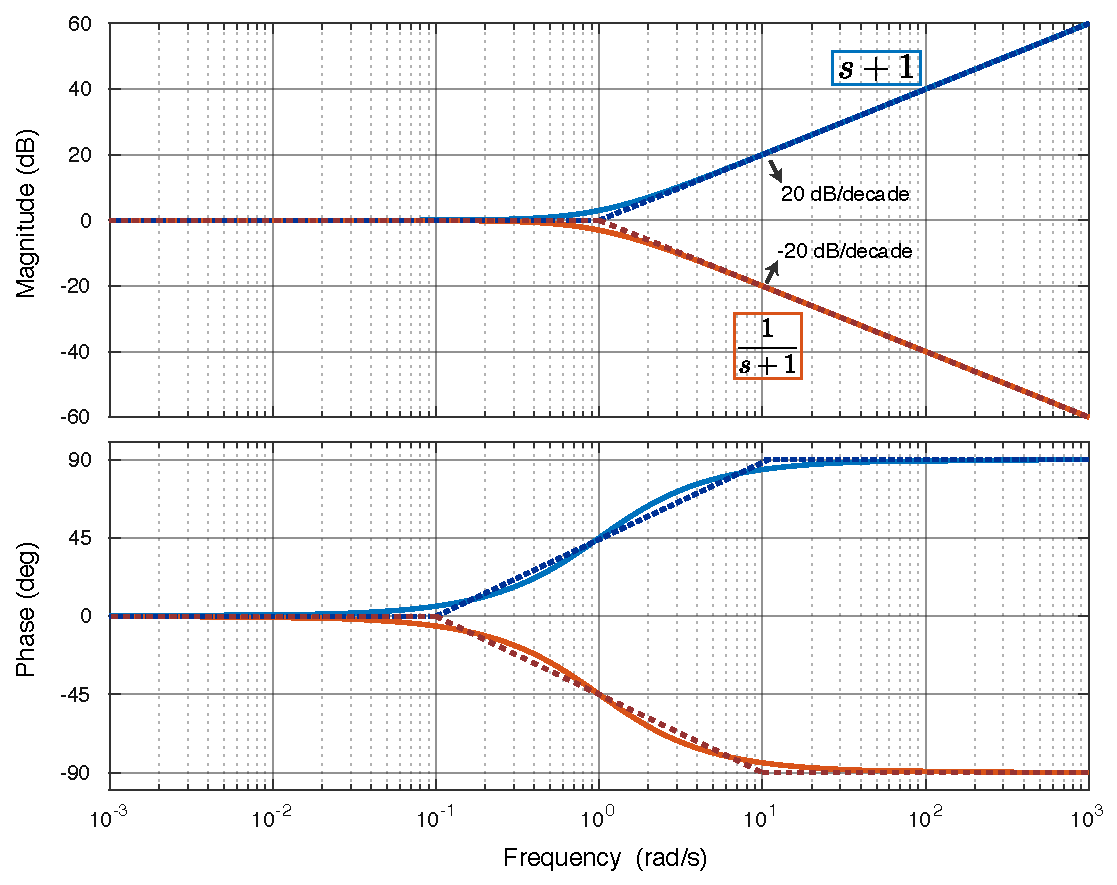
\includegraphics[width=0.9\textwidth]{sp1}
    \end{center}
  \end{minipage}

\vspace{6 pt}

Now let's analyze the phase and magnitude (dB) response of 
%
\begin{align*}
  G(s) = T s + 1 = \frac{s + a}{a} \ \mathrm{where} \ a = \frac{1}{T}
\end{align*}
%
Magnitude and phase functions can be obtained as
\begin{align*}
  M_{dB}  &= 20 \, \mathrm{log}_{10} | G( j \omega) | = 20 \, \mathrm{log}_{10} \left( T^2 \omega^2 + 1 \right)^{1/2} = 10 \, \mathrm{log}_{10} \left( T^2 \omega^2 + 1 \right)
  \\
  \phi &= \arctan T \omega                                    
\end{align*}
%
If we follow a similar approach, we can approximate the gain curves as
%
\begin{align*}
  \mathrm{Low-Frequency}: \omega \leq \frac{1}{T} = a  \ \Rightarrow \ M_{dB}  &\approx 0 \ \mathrm{dB} \\
  \mathrm{High-Frequency}: \omega \geq \frac{1}{T} = a \ \Rightarrow \ M_{dB}  &\approx 20 \, \mathrm{log}_{10} ( T \omega )
\end{align*}
%
Note that high-frequency and low-frequency approximations intersect at
$\omega = a \ rad/s = \frac{1}{T} \ rad/s$ and $M_{dB} = 0 \ \mathrm{dB}$ point. Now 
let's approximate the phase response
%
\begin{align*}
  \mathrm{Low-Frequency}: \omega \leq \frac{0.1}{T} = 0.1 a \ \Rightarrow \ \phi  &\approx 0^o  \\
  \mathrm{High-Frequency}: \omega \geq \frac{10}{T} = 10 a  \ \Rightarrow \ \phi &\approx 90^o \\
  \mathrm{Medium-Frequency} \ \Rightarrow \ \phi & \approx 45^0 + 45^0 \mathrm{log}_{10} ( \omega)
\end{align*}
%
Note that low-frequency and mid-frequency approximations intersect
when $\omega = 0.1 a \ rad/s$,
whereas high-frequency and mid-frequency approximations intersect when
$\omega = 10 a \ rad/s$.
The corner freqency of this system is $\omega_c = a \ rad/s = 1/T \
rad/s$. Note that in order to obtin the bode plot of $T s + 1$, we
simply shift the bode plot of $s + 1$ (in $\omega$ axis). 

\vspace{6pt}

\textbf{Ex:} The figure below
illustrates the original bode plots (solid curves) of $G_1(s) = (s+10)$ and $G_2(s) = \frac{1}{s+10}$ as well as
their approximations (dashed lines). 

\vspace{6 pt}

  \begin{minipage}[h]{1\linewidth}
    \begin{center}
      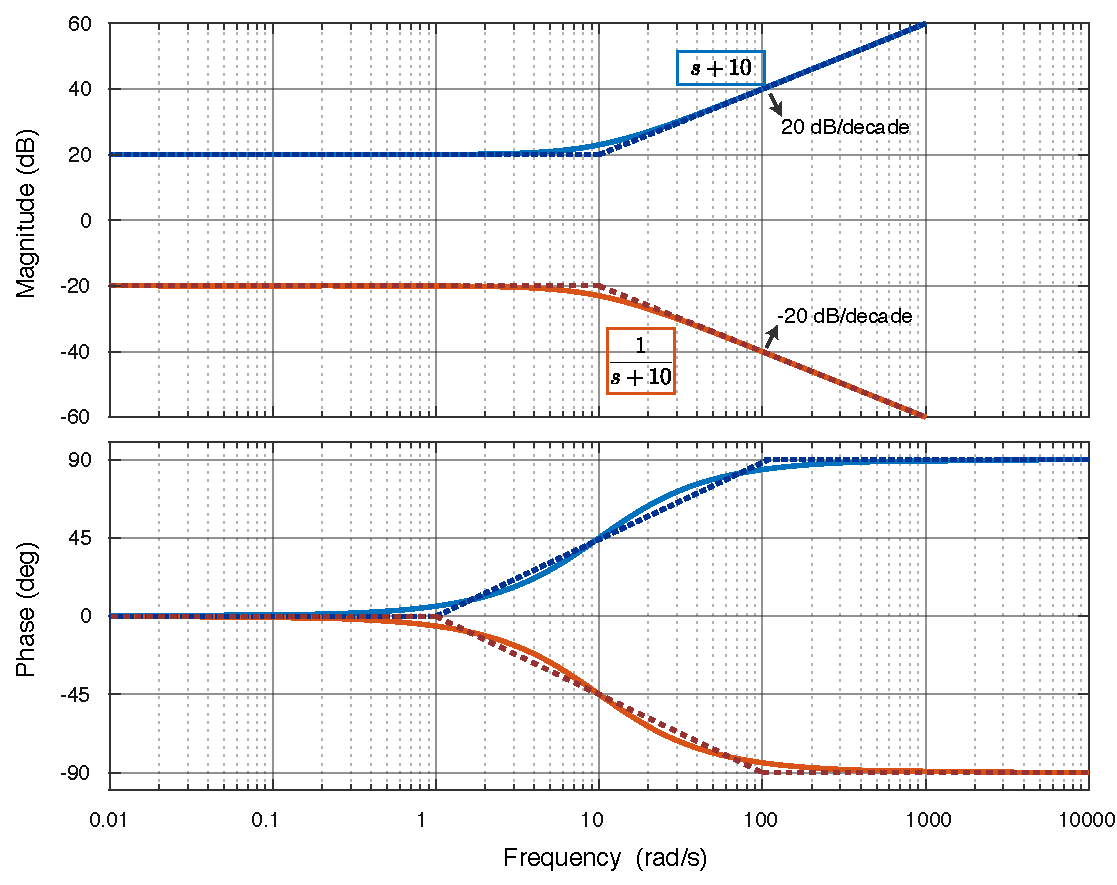
\includegraphics[width=0.9\textwidth]{spa}
    \end{center}
  \end{minipage}

\vspace{6 pt}

\subsection*{Bode Plots of Second-Order Forms}

A unity gain standard second order system can be written in the form
%
\begin{align*}
	G(s) = \frac{\omega_n^2}{s^2 + 2 \zeta \omega_n s + \omega_n^2} 
		= \frac{1}{\frac{1}{\omega_n^2} s^2 + \frac{2 \zeta}{\omega_n} s + 1} 
\end{align*}
%
\textbf{Case 1 : $\zeta = 1$} First let's analyze the bode plots for the critically damped case, 
%
\begin{align*}
	G(s) =  \frac{1}{\frac{1}{\omega_n^2} s^2 + \frac{2 \zeta}{\omega_n} s + 1} 
		= \frac{1}{(\frac{s}{\omega_n} + 1)^2}
\end{align*}
%
We can easily observe that 
%
Magnitude and phase functions can be obtained as
\begin{align*}
  M_{dB} \lbrace G(s) \rbrace &= 20 \, \mathrm{log}_{10} | G( j \omega) | =   20 \, \mathrm{log}_{10} \left| \frac{1}{\frac{s}{\omega_n} + 1} \right|^2
  \\
  	&= 2 M_{dB} \left\lbrace \frac{1}{\frac{s}{\omega_n} + 1}  \right\rbrace
	\\  
  \phi \lbrace G(s) \rbrace &= 2 \phi \left\lbrace \frac{1}{\frac{s}{\omega_n} + 1}  \right\rbrace
\end{align*}

\textbf{Ex:} The figure below
illustrates the original bode plots (solid curves) of $G_1(s) = \frac{10}{s+10}$ and $G_2(s) = \frac{100}{(s+10)^2}$ as well as
their approximations (dashed lines). 

\vspace{6 pt}

  \begin{minipage}[h]{1\linewidth}
    \begin{center}
      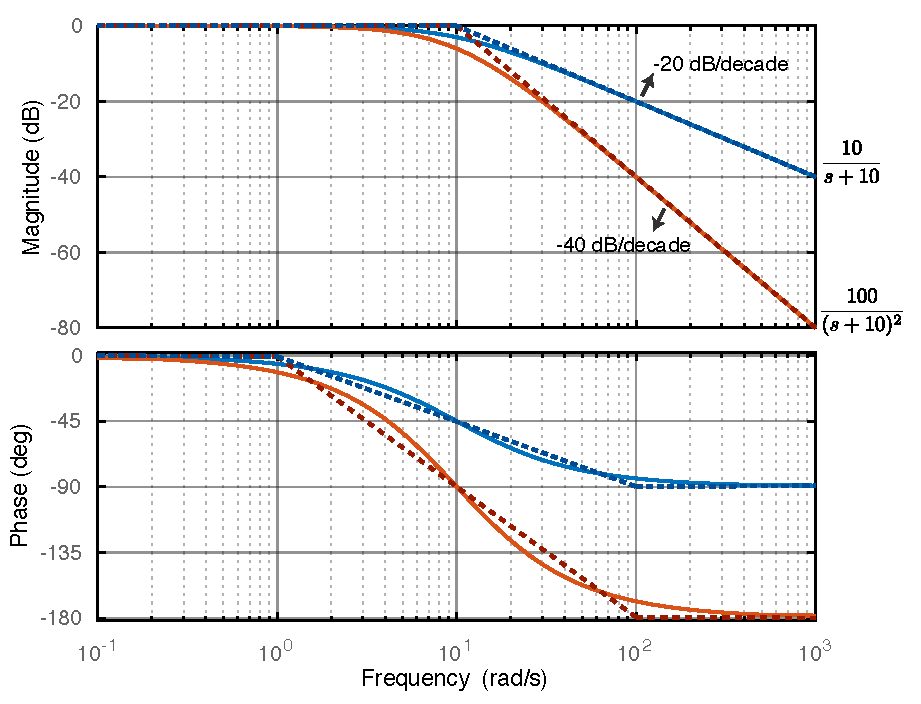
\includegraphics[width=0.9\textwidth]{second}
    \end{center}
  \end{minipage}

\vspace{6 pt}

\textbf{Case 2: $\zeta > 1$} Over-damped case is simply the combination of two identical first order
systems. 

\textbf{Ex:}  Let's analyze the the bode plots for the following system
%
\begin{align*}
	G(s) =  \frac{10}{(s+1)(s+10)}
		= \frac{1}{ s + 1 } \frac{10}{ s + 10 }
\end{align*}
%
We can easily observe that 
\begin{align*}
  M_{dB} \lbrace G(s) \rbrace &= M_{dB} \left\lbrace \frac{1}{s+1}  \right\rbrace +
   M_{dB} \left\lbrace \frac{10}{s+10}  \right\rbrace
	\\  
  \phi \lbrace G(s) \rbrace &= \phi \left\lbrace \frac{1}{s + 1}  \right\rbrace + 
   \phi \left\lbrace \frac{10}{s + 10}  \right\rbrace 
\end{align*}
%
The figure below
illustrates the original bode plots (solid curves) of $G_1(s) = \frac{1}{s+1}$, $G_2(s) = \frac{10}{s+10}$ and $G_4(s) = \frac{10}{(s+1) (s+10)}$ as well as their approximations (dashed lines). 

\vspace{6 pt}

  \begin{minipage}[h]{1\linewidth}
    \begin{center}
      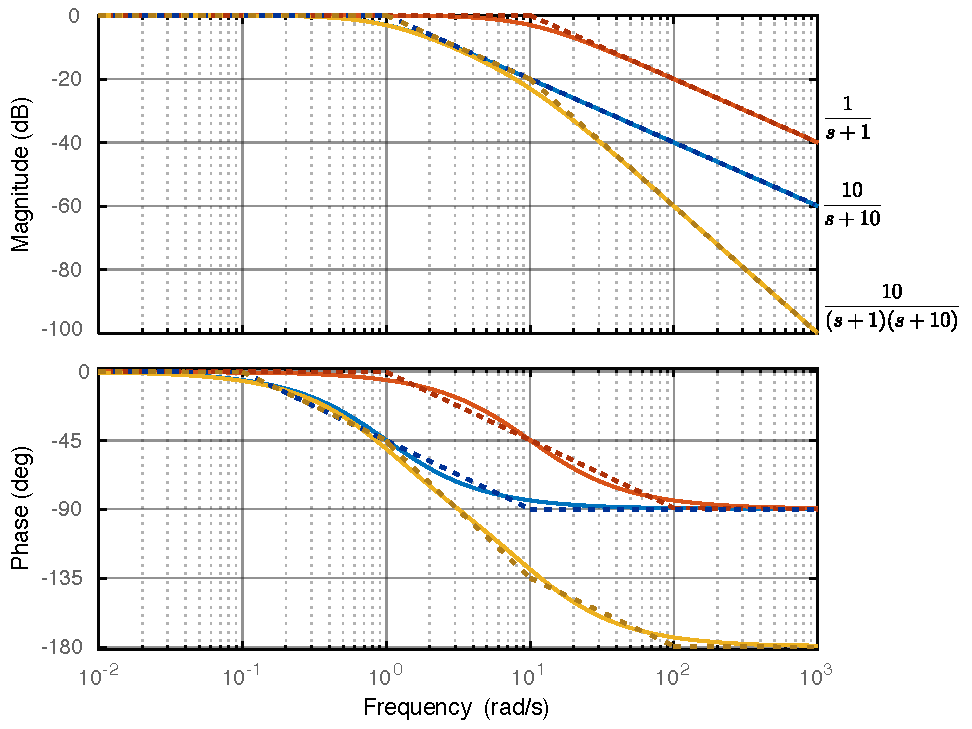
\includegraphics[width=0.9\textwidth]{over}
    \end{center}
  \end{minipage}

\newpage

\textbf{Case 3 : $\zeta < 1$} For under-damped systems, corner frequencies 
of the piece-wise linear approximations are unchanged. Thus, we use same 
approximation with the critically damped case. However, as damping ratio 
increases we may observe larger differences between the actual bode plot
and the approximations. 

\textbf{Ex:} The figure below
illustrates the original bode plots (solid curves) of $G_1(s) = \frac{10}{s+10}$ and $G_2(s) = \frac{100}{(s+10)^2}$ as well as
their approximations (dashed lines). 

\vspace{6 pt}

  \begin{minipage}[h]{1\linewidth}
    \begin{center}
      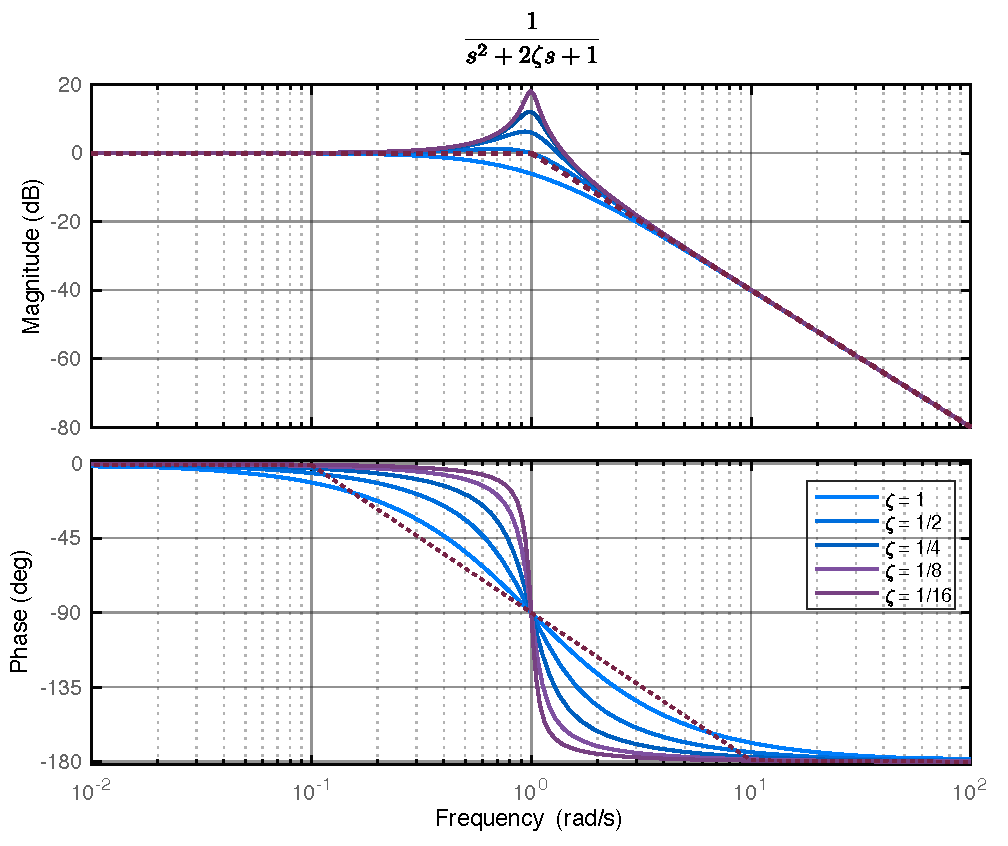
\includegraphics[width=0.9\textwidth]{under}
    \end{center}
  \end{minipage}

\vspace{6 pt}

We can see that best phase matching between the actual bode plot and approximation is achieved when
$\zeta = 1$, however surprisingly best magnitude matching between the actual bode plot and approximation is achieved when
$\zeta = 2$. Indeed, best match between the actual and approximate bode plots in magnitude is achieved when $\zeta = 1/\sqrt{2}$. 

\newpage

\section{Gain \& Phase Margin from Bode Plots}

We already know that for a feedback system, phase and 
gain margins can be computed based on the Frequency Response
characteristics of the open-loop transfer function, $G_{OL}(j \omega)$ (under
some assumption regarding the system properties).

Specifically, we can compute the phase crossover frequency, $\omega_{pc}$ and the gain margin, 
$g_m$ (linear scale) and $G_m$ (dB scale), as
%
\begin{align*}
  \angle [ G_{OL}(j \omega_{p}) ] &= \pm -180^0
  \quad \Rightarrow \quad
  g_m = \frac{1}{| G_{OL}(j \omega_{pc})| } \quad \mathrm{or} \quad G_m
  = -20 \, \mathrm{log}_{10} | G_{OL}(j \omega_{pc} ) |
\end{align*}
%
where as gain crossover frequency, $\omega_{gc}$, and the 
phase margin can be computed as
%
\begin{align*}
  | G_{OL}(j \omega_{gc}) | &= 1 \quad \mathrm{or} \quad 
  M_{dB} \lbrace G_{OL}(j \omega_{gc}) \rbrace = 0 \ \mathrm{dB}
   \quad \Rightarrow \quad
  \phi_m = \pi + \angle G_{OL} (j \omega_{gc})
\end{align*}
% 
Indeed it is generally easier to derive the phase and gain margin of
a system from the bode plots compared to the Nyquist \& polar plots.

\textbf{Ex:} Compute the phase margin 
for the following closed-loop system for $K = 2$ and $K = 4$,
both from the approximate and actual bode plots. 

\begin{center}
\begin{minipage}[h]{\linewidth}
    \begin{center}
      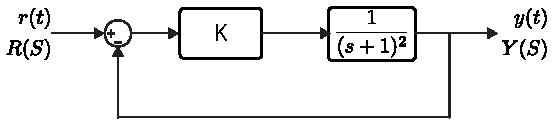
\includegraphics[width=0.45\textwidth]{ex2block}
    \end{center}
\end{minipage}
\end{center}

Actual bode plots for both gains are illustrated
below. 

\begin{center}
\begin{minipage}[h]{\linewidth}
    \begin{center}
      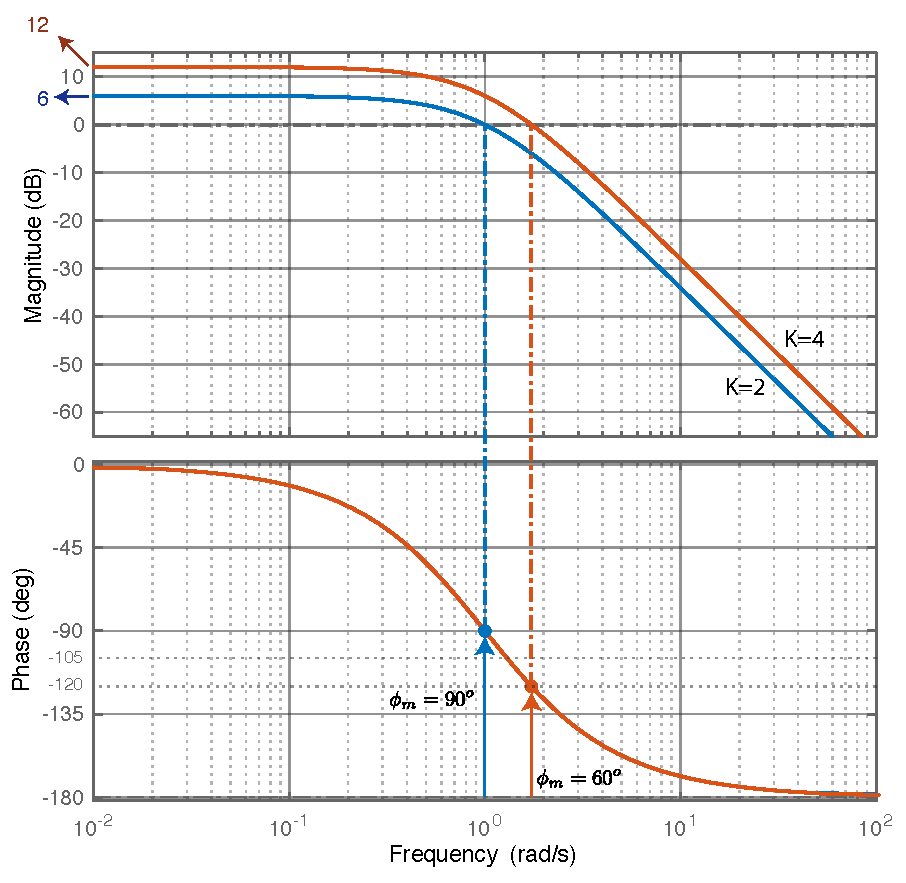
\includegraphics[width=0.7\textwidth]{marginactual}
    \end{center}
\end{minipage}
\end{center}

If we label the gain crossover frequencies and find the 
corresponding phase values, we can easily compute the phase 
margins as
%
\begin{align*}
  K &= 2 \Rightarrow \phi_m = 90^o \quad (\omega_{gc} = 1 \ rad/s)
  \\
  K &= 4 \Rightarrow \phi_m = 60^o \quad (\omega_{gc} \approx 1.8 \ rad/s)
\end{align*}
%
These results verify the actual phase margin values that we previously computed
using the Nyquist plot. Note that $G_m$ is infinity for both cases.

Now let's illustrate the approximate bode plots (dashed lines),
which are illustrated in the Figure below on top of the actual ones

\begin{center}
\begin{minipage}[h]{\linewidth}
    \begin{center}
      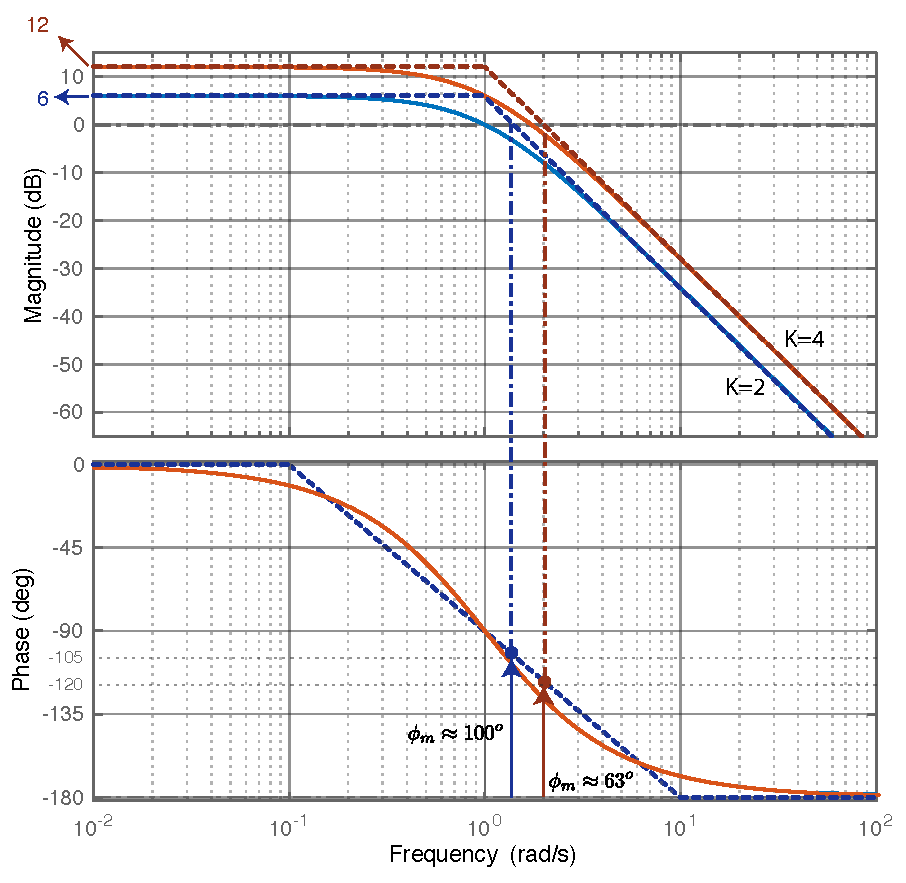
\includegraphics[width=0.7\textwidth]{margin}
    \end{center}
\end{minipage}
\end{center}

If we approximately compute the phase margins based
on the approximate bode plots we obtain that 
%
\begin{align*}
  K &= 2 \Rightarrow \phi_m \approx 100^o 
  \\
  K &= 4 \Rightarrow \phi_m \approx 63^o 
\end{align*}

\vspace{12pt}

\textbf{Ex:} Compute the gain margin and phase margin 
for the following closed-loop system for $K = 1$ and $K = 8$
both from the actual and approximate bode plots. 

\begin{center}
\begin{minipage}[h]{\linewidth}
    \begin{center}
      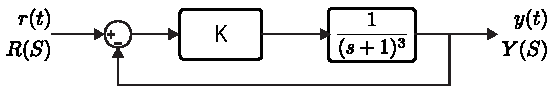
\includegraphics[width=0.5\textwidth]{ex3block}
    \end{center}
\end{minipage}
\end{center}

First let's analyze $K = 1$, the Figure below illustrates the
actual and approximate bode plots of $G(s) = \frac{1}{(s+1)^3}$.

\begin{center}
\begin{minipage}[h]{\linewidth}
    \begin{center}
      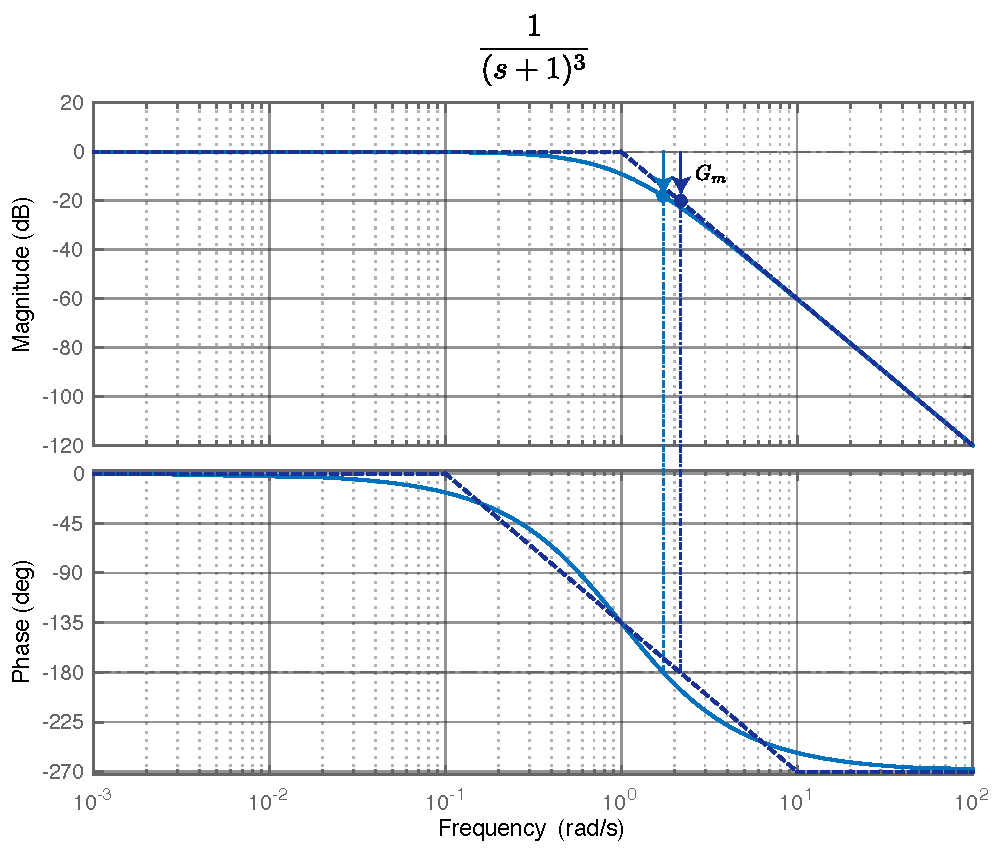
\includegraphics[width=0.75\textwidth]{margin2}
    \end{center}
\end{minipage}
\end{center}

We can see that phase margin is $180^o$ for the given system,
since $\omega_{gc} = 0 \ \rightarrow \ \phi (\omega_{gc} ) = 0^o$. 
On the other hang we can derive the following gain margin estimates
from the actual and approximate bode plots
%
\begin{align*}
	&\mathrm{Actual:} \quad G_m \approx 18 \ \mathrm{dB} \quad \rightarrow \quad g_m \approx 8	
	\\
	&\mathrm{Approximate:} \quad G_m \approx 20 \ \mathrm{dB} \quad \rightarrow \quad g_m \approx 10
\end{align*}
%
Now let's analyze $K = 8$, the Figure below illustrates the
actual Bode plots of $G(s) = \frac{8}{(s+1)^3}$.


\begin{center}
\begin{minipage}[h]{\linewidth}
    \begin{center}
      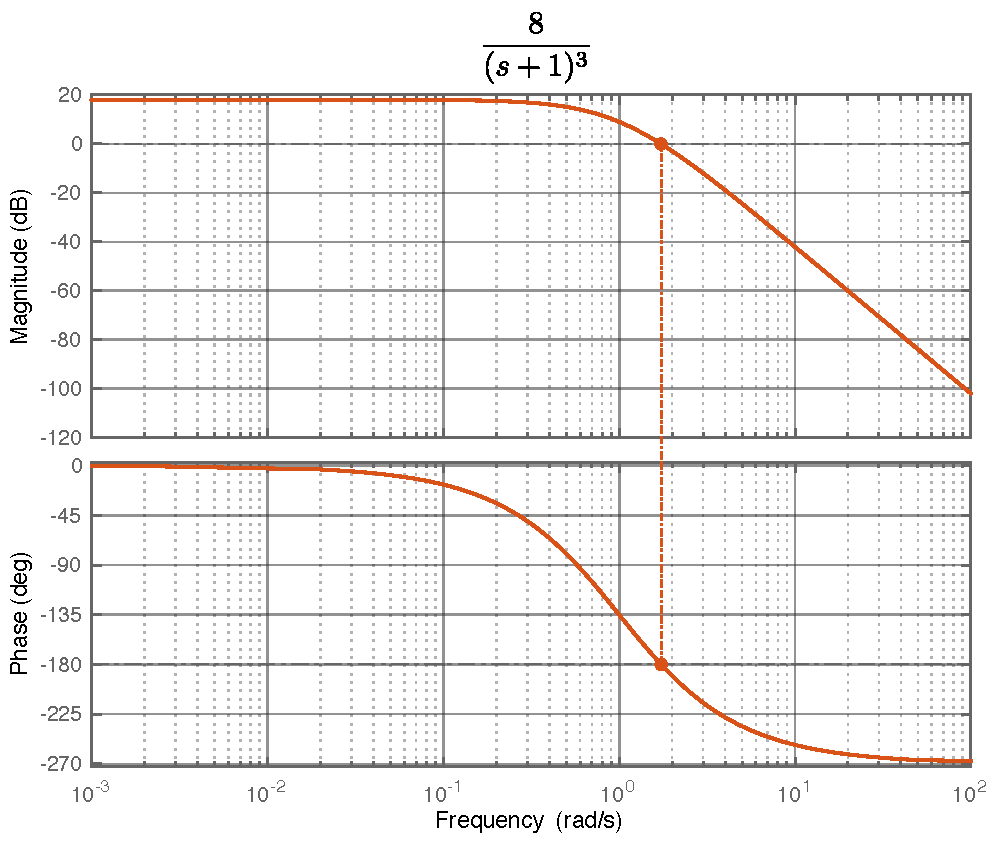
\includegraphics[width=0.7\textwidth]{margin3actual}
    \end{center}
\end{minipage}
\end{center}

We can see from the actual bode-plot that  $G_m =  0 \ \mathrm{dB}$
and $\phi_m = 0^o$.
However, if we draw the approximate bode plots 

\begin{center}
\begin{minipage}[h]{\linewidth}
    \begin{center}
      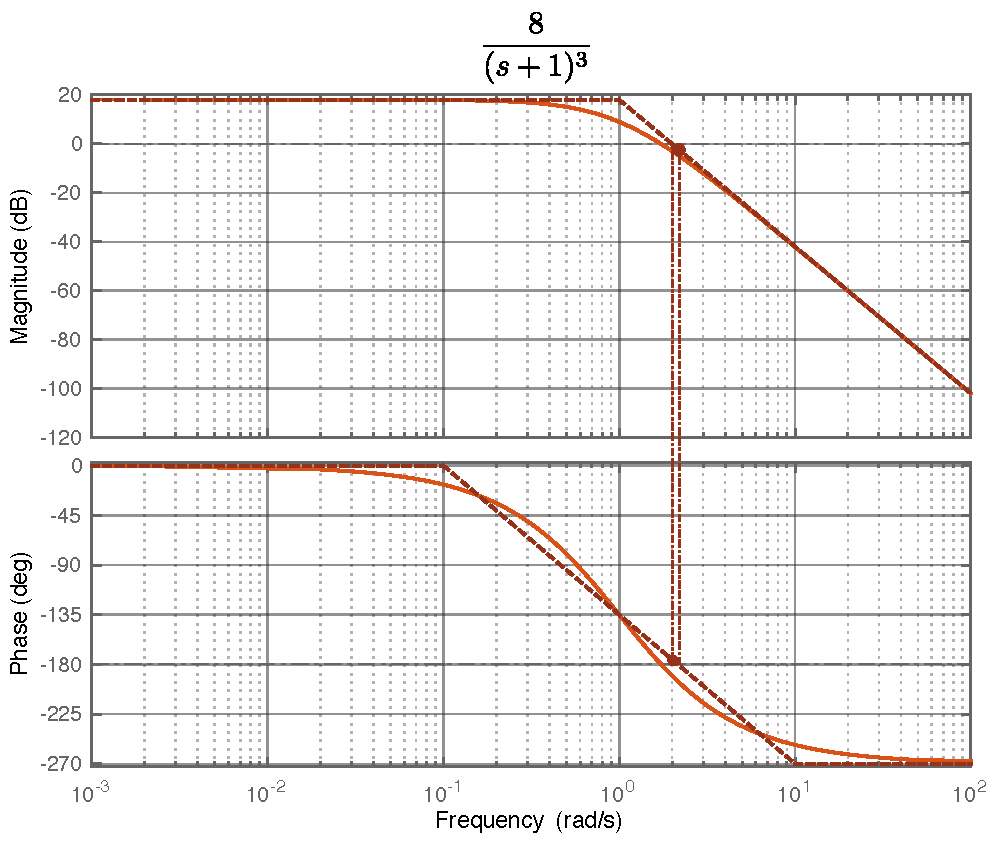
\includegraphics[width=0.7\textwidth]{margin3}
    \end{center}
\end{minipage}
\end{center}

and estimate these margins we obtain
%
\begin{align*}
	&G_m \approx 2 \ \mathrm{dB} \quad \rightarrow \quad g_m \approx 1.2	
	\\
	&\phi_m = 2^o
\end{align*}
%
If we consider the bode plots that we draw based on asymptotic approximations and compute the phase and gain margins, we can assume that system is indeed stable. However, these margins are rather low. In this respect, we can conclude that if one analyzes the absolute stability of a system using approximately bode plots, in order to comment on stability, he/she should observe significant phase and gain margins.

\textbf{Ex:} Compute  phase margin for the following closed-loop system 
using the actual and approximate bode plots

\begin{center}
\begin{minipage}[h]{\linewidth}
    \begin{center}
      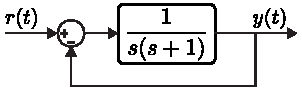
\includegraphics[width=0.3\textwidth]{ex4block}
    \end{center}
\end{minipage}
\end{center}

The Figure below illustrates the actual and approximate bode plots.

\begin{minipage}[h]{1\linewidth}
    \begin{center}
      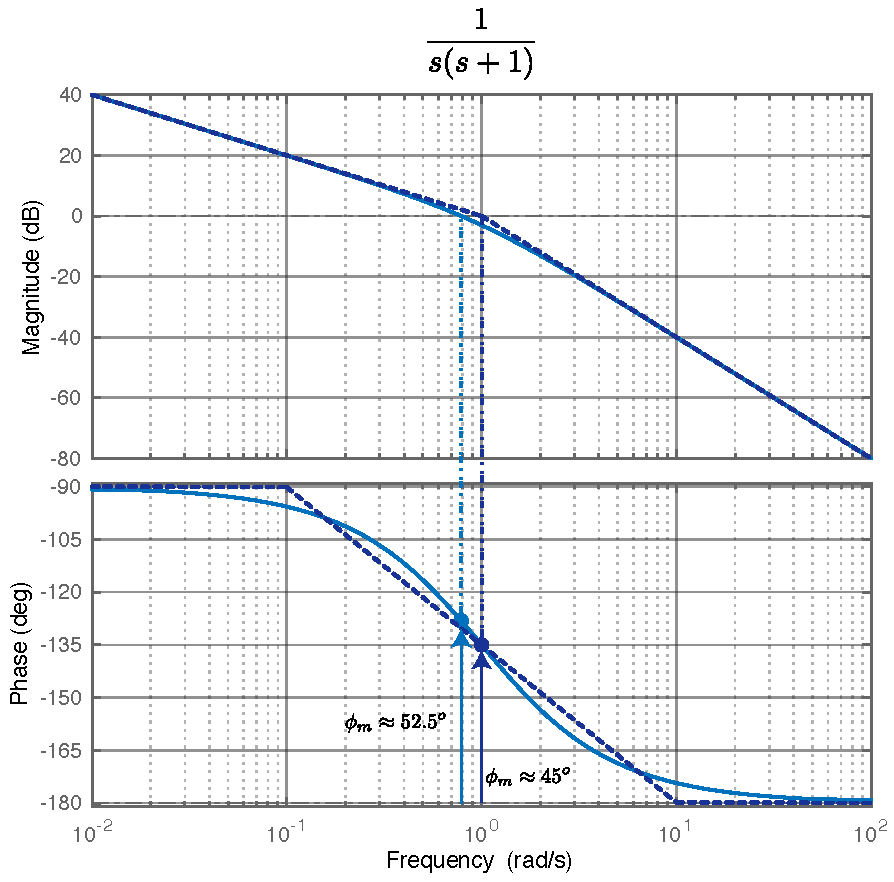
\includegraphics[width=0.75\textwidth]{type1}
    \end{center}
\end{minipage}

We can derive the following phase margin computations from the
actual and approximate bode plots
%
%
\begin{align*}
	&\mathrm{Actual:} \quad \phi_m \approx 52.5^0 \quad (\omega_{gc} \approx 0.8 \ rad/s)
	\\
	&\mathrm{Approximate:} \quad \phi_m \approx 45^o \quad (\omega_{gc} = 1 \ rad/s)
\end{align*}
%



% **** This ENDS THE EXAMPLES. DON'T DELETE THE FOLLOWING LINE:
\end{document}